% Combined Beamer Slides: Introduction to LLMs
\documentclass[german,10pt]{beamer}
\usepackage{tcolorbox}
\usepackage{bm}
\usepackage{graphicx} \graphicspath{ {./figs/} }
%% Integer set
\newcommand{\field}[1]{\mathbb{#1}}
\newcommand{\Rset}{\field{R}}
\newcommand{\Zset}{\field{Z}}
\newcommand{\Qset}{\field{Q}}
\newcommand{\Nset}{\field{N}}


\usetheme{Madrid}
\usecolortheme{seagull}
\usepackage{tikz}
\usepackage{booktabs}
\usepackage{hyperref}
% Beamer specific settings
\mode<presentation>
{
  \usetheme{Boadilla} % Without index, with footer
}

\title{CE 401/5501: Introduction to Large Language Models}
\subtitle{It is just more than prompting and chatting!}
\author[]{Professor ZhiQiang Chen}
\institute[UMKC]{School of Science and Engineering \\ University of Missouri-Kansas City}
\date{}

% Outline at each section start
\AtBeginSection[]{
  \begin{frame}<beamer>\frametitle{Outline}
    \tableofcontents[currentsection,currentsubsection]
  \end{frame}
  \begin{frame}[plain]
    \centering
    \vfill
    {\usebeamerfont{section title}\insertsectionhead\par}
    \vfill
  \end{frame}
}

\setbeamersize{text margin left=1cm}
\setbeamersize{text margin right=1cm}

\begin{document}

% Title Slide
\begin{frame}
  \titlepage
\end{frame}


% Section II: Classical NLP: Pre-Transformer Era
\section{Classical NLP: Pre-Transformer Era}

% Separation Title Page for Classical NLP
\begin{frame}[plain]
  \centering
  {\Huge Classical NLP}\vspace{0.5cm}\\
  {\Large Pre-Transformer Era}
\end{frame}

% Slide 1: Early Machine Translation Vision
\begin{frame}{Early Machine Translation Vision}
  \begin{itemize}
    \item 1949: Warren Weaver’s Memorandum—analogy to cryptography and information theory
    \item 1954: Georgetown–IBM experiment translating Russian to English
    \item Coined notion: translation as statistical decoding of language codes
  \end{itemize}
\end{frame}

% Slide 2: Rule-Based and Linguistic Models
\begin{frame}{Rule-Based and Linguistic Models}
  \begin{itemize}
    \item 1960s–70s: Expert systems and grammar formalisms (Chomskyan generative grammar)
    \item Symbolic parsers, feature unification, hand-crafted lexicons
    \item Limitations: brittle, resource-intensive development
  \end{itemize}
\end{frame}

% Slide 3a: Statistical NLP Emergence
\begin{frame}{Statistical NLP Emergence}
  \begin{itemize}
    \item 1980s–90s: N-gram language models, trained from corpora (\textit{corpus})
    \item Hidden Markov Models for POS tagging and speech recognition
      \begin{itemize}
        \item Part-of-Speech (POS) tagging assigns each word to grammatical categories
      \end{itemize}
    \item 1990s: IBM Models 1–5 for statistical machine translation (Brown et al.)
      \begin{itemize}
        \item Model translation probabilities: lexical, positional, fertility, reordering
      \end{itemize}
    \item 2003: Phrase-based Statistical machine translation (SMT) (Koehn et al.)
  \end{itemize}
\end{frame}

% Slide 3b: Neural NLP Emergence
\begin{frame}{Neural NLP Emergence}
  \begin{itemize}
    \item Early 2000s: RNNs for language modeling; suffered from vanishing gradients
    \item 1997: LSTM networks introduced (Hochreiter \& Schmidhuber)
      \begin{itemize}
        \item Solved vanishing-gradient problem, enabled long-range context modeling
        \item Adopted in language modeling, speech recognition, early NMT
      \end{itemize}
    \item 2014: Seq2Seq with Attention (Sutskever et al.) marks first neural MT breakthroughs
  \end{itemize}
\end{frame}

% Slide 4: Milestones Timeline
\begin{frame}{Milestones Timeline}
  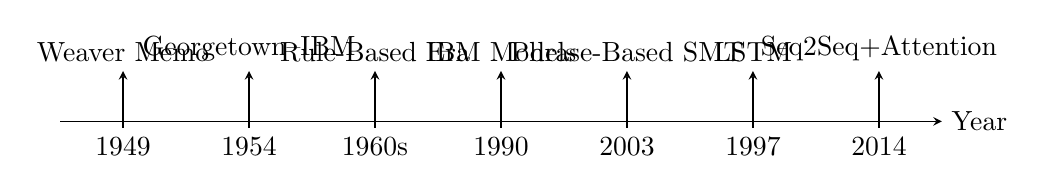
\begin{tikzpicture}[>=stealth,scale=0.8]
    % Timeline baseline
    \draw[->] (0,0) -- (14,0) node[right]{Year};
    % Milestone ticks and vertical arrows with labels
    \foreach \x/\label/\desc in {
      1/1949/Weaver Memo,
      3/1954/Georgetown–IBM,
      5/1960s/Rule‑Based Era,
      7/1990/IBM Models,
      9/2003/Phrase‑Based SMT,
      11/1997/LSTM,
      13/2014/Seq2Seq+Attention
    } {
      \draw (\x,0.1) -- (\x,-0.1) node[below]{\label};
      \draw[->] (\x,0) -- (\x,0.8) node[above]{\desc};
    }
  \end{tikzpicture}
\end{frame}




% Section I: Basics of LLMs
\section{Basics of Transformer-based Large Language Models}
% LLM Scale & Benchmark Performance

% Transition into LLM Section
\begin{frame}{Why Large Language Models?}
  \begin{itemize}
    \item \textbf{From Task‑Specific to General‑Purpose:}  
      Earlier neural NLP models (RNNs, LSTMs, Seq2Seq) excelled at individual tasks, but required separate architectures and training for each.  
    \item \textbf{Unified Pretraining Paradigm:}  
      LLMs leverage massive unsupervised pretraining to capture grammar, facts, and even \textit{ reasoning} in one model.  
    \item \textbf{Emergent Capabilities:}  
      At scale, simple next‑token prediction yields zero‑/few‑shot learning, in‑context adaptation, and cross‑task generalization.
    \item \textbf{Key Enabler:}  
      The Transformer’s self‑attention mechanism—fully parallelizable and capable of modeling long‑range dependencies—forms the backbone of every state‑of‑the‑art LLM.  
  \end{itemize}
\end{frame}


\begin{frame}{LLM Scale \& Benchmark Performance}
  \begin{table}[h!]
    \centering
    \begin{tabular}{lcc}
      \hline
      \textbf{Model} & \textbf{Parameters} & \textbf{MMLU (5-shot)} \\
      \hline
      GPT-3 & 175B & 46.4\% \\
      Chinchilla & 70B & 67.5\% \\
      PaLM & 540B & 69.3\% \\
      LLaMA (65B) & 65B & 63.4\% \\
      GPT-4 & 1.76T  & 86.4\% \\
      \hline
    \end{tabular}
    \caption{Scale and MMLU performance of major LLMs}
  \end{table}
  \vspace{0.5em}
  {\footnotesize Sources: Brown et al. (2020); Rae et al. (2022)} 
\end{frame}


% Slide: LLM Architecture Workflow (Output Block to the Side)
\begin{frame}{LLM Architecture Workflow}
  \small
  \centering
  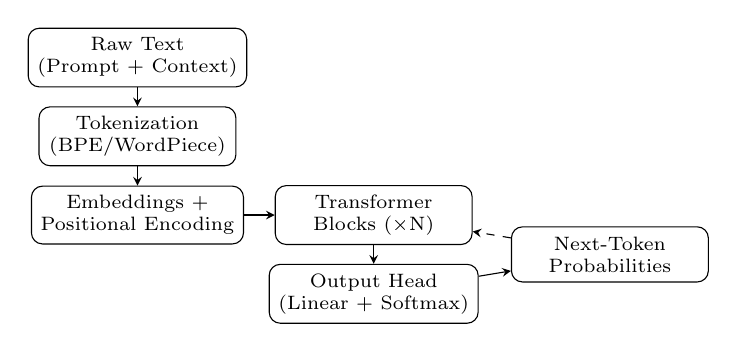
\begin{tikzpicture}[>=stealth,font=\scriptsize]
    \tikzset{box/.style={
      draw, rounded corners, minimum width=2.5cm, minimum height=0.7cm, align=center
    }}
    % Left column
    \node[box] (input)       at (0,0)        {Raw Text\\(Prompt + Context)};
    \node[box] (token)       at (0,-1)       {Tokenization\\(BPE/WordPiece)};
    \node[box] (embed)       at (0,-2)       {Embeddings +\\Positional Encoding};
    % Middle column
    \node[box] (transformer) at (3,-2)       {Transformer\\Blocks (×N)};
    \node[box] (head)        at (3,-3)       {Output Head\\(Linear + Softmax)};
    % Side column for looped output
    \node[box] (output)      at (6,-2.5)     {Next‑Token\\Probabilities};

    % Arrows
    \draw[->] (input)       -- (token);
    \draw[->] (token)       -- (embed);
    \draw[->] (embed)       -- (transformer);
    \draw[->] (transformer) -- (head);
    \draw[->] (head)        -- (output);
    \draw[dashed,->] (output) -- (transformer);

  \end{tikzpicture}

  \vspace{0.5em}
  {\footnotesize Dashed arrow indicates the autoregressive feedback loop.}
\end{frame}









% Slide: Tokenization (Example)
\begin{frame}{Tokenization}
  \textbf{Example:} “ChatGPT revolutionizes NLP.”  
  \vspace{0.5em}
  \begin{itemize}
    \item \textbf{Byte‑Pair Encoding (BPE)} splits into subword tokens:  
      \[
        [\,\text{"Chat"}, \text{"GP"}, \text{"T"}, \text{" revolution"}, \text{"izes"}, \text{" NLP"}, \text{"."}\,]
      \]
    \item Balances vocabulary size and coverage by merging frequent pairs.
  \end{itemize}
\end{frame}

% Slide: Embeddings (Dimensions & Space)
\begin{frame}{Embeddings}
  \begin{itemize}
    \item \textbf{Lookup}: 
      \[
        \mathbf{e}_i = E\,\mathrm{one\_hot}(x_i), 
        \quad x_i\in\{1,\dots,|\mathcal{V}|\}
      \]
    \item \textbf{Embedding matrix}: 
      \[
        E\in\mathbb{R}^{|\mathcal{V}|\times d}, \quad \mathbf{e}_i\in\mathbb{R}^d
      \]
    \item \textbf{Modern GPT example}:  
      \[
        |\mathcal{V}| \approx 50{,}257,\quad d = 12{,}288
      \]
    \item \textbf{Matrix size}:  
      \[
        50{,}257 \times 12{,}288 \approx 619\,\text{million parameters}
      \]
  \end{itemize}
\end{frame}
% Slide: Why Is the Embedding Dimension So Large?
\begin{frame}{Why Such a Large Embedding Dimension?}
  \begin{itemize}
    \item \textbf{Capacity for Nuance}:  
      Higher \(d\) allows each token to be represented with fine‐grained features capturing syntax, semantics, and even world knowledge.  
    \item \textbf{Model Depth Alignment}:  
      Embedding dimension typically matches the hidden size of the Transformer (e.g.\ 12,288), ensuring seamless residual connections and multi‑head projections.  
    \item \textbf{Empirical Performance}:  
      Scaling laws show that increasing \(d\) improves downstream zero‑/few‑shot accuracy up to a point, especially for very large corpora.  
    \item \textbf{Trade‑Off}:  
      \(\uparrow d\) \(\implies\) \(\uparrow\) parameter count and compute cost, but also \(\uparrow\) representational flexibility.
  \end{itemize}
\end{frame}

% Slide: Sparsity of the Embedding Space
\begin{frame}{Sparsity of the Embedding Space}
  \small
  \begin{itemize}
    \item Vocabulary size $\lvert\mathcal V\rvert \approx 50{,}257$ tokens embedded in $\mathbb R^{12{,}288}$.
    \item Even if each coordinate is stored as a 16‑bit float, the total representable vectors $\sim2^{16\times d}$ vastly exceeds $\lvert\mathcal V\rvert$:  
      \[
        \frac{\lvert\mathcal V\rvert}{2^{16\,d}}\approx 0\quad(\text{practically zero occupancy})
      \]
    \item Embedding vectors are \emph{dense} (almost all $d$ coordinates nonzero) but occupy a tiny, low‑dimensional manifold within $\mathbb R^d$.
    \item Even considering all correlated tokens (i.e., the entire scope of human knowledge), their embeddings still lie on a sparse manifold far smaller than the full space.
    \item Consequence: token vectors are nearly orthogonal (average cosine similarity $\approx0.02$), maximizing representational capacity.
  \end{itemize}
\end{frame}





% Slide 3: Transformer Overview
\begin{frame}{Transformer Overview}
  \begin{itemize}
    \item Architectures: Encoder-only, Decoder-only (e.g., GPT), and Encoder-Decoder
    \item GPT uses a stack of decoder-only blocks
    \item Each block: self-attention + feedforward + residual connections
  \end{itemize}
  \begin{figure}
      \centering
      
\includegraphics[width=0.7\linewidth]{figs/transformer-llm.png}
      \caption{LLM's typical stacked decoder blocks.}
      \label{fig:enter-label}
  \end{figure}
\end{frame}

% Slide: Transformer Architecture & Its Significance
\begin{frame}{Transformer Architecture \& Its Significance}
  \begin{columns}[t]
    \column{0.48\textwidth}
      \textbf{Transformer Architecture}
      \begin{itemize}
        \item \textbf{Multi‑Head Self‑Attention}: captures global token dependencies
        \item \textbf{Positional Encodings}: inject sequence order information
        \item \textbf{Feed‑Forward Networks}: two-layer MLP per position
        \item \textbf{Residual \& LayerNorm}: stabilize and speed up deep training
        \item \textbf{Parallelizable}: processes all tokens simultaneously (no recurrence)
      \end{itemize}

    \column{0.48\textwidth}
      \textbf{Significance}
      \begin{itemize}
        \item \textbf{Efficient Scaling}: parallelism enables training on massive corpora
        \item \textbf{Long‑Range Context}: attention spans entire input sequence
        \item \textbf{Pretrain\& Fine‑Tune}: foundation for transfer learning workflows
        \item \textbf{LLM Foundation}: underpins GPT, BERT, and myriad variants
        \item \textbf{Emergent Behaviors}: supports zero‑/few‑shot learning and adaptivity
      \end{itemize}
  \end{columns}
\end{frame}

% Slide: Self‑Attention Mechanism (Updated)
\begin{frame}{Self‑Attention Mechanism}
  {\small
  \[
    \mathrm{Attention}(Q,K,V)
    = \mathrm{softmax}\!\Bigl(\tfrac{QK^\top}{\sqrt{d_k}}\Bigr)\,V
    \quad\text{where}\quad
    Q = XW^Q,\,
    K = XW^K,\,
    V = XW^V
  \]
  \[
    \text{head}_h = \mathrm{Attention}(XW_h^Q,\,XW_h^K,\,XW_h^V),\quad
    \mathrm{MultiHead}(X) = \mathrm{Concat}(\text{head}_1,\dots,\text{head}_H)\,W^O
  \]
  }
  \vspace{-0.5em}
  \begin{itemize}
    \item Scaled dot‑product avoids extremely large logits when $d_k$ is large.
    \item Multi‑head attention splits $d$ into $H$ subspaces ($d_k = d/H$), then recombines.
    \item Residual \& LayerNorm wrap each sublayer:
      \(\,Z' = \mathrm{LayerNorm}(X + \mathrm{MultiHead}(X))\).
  \end{itemize}
\end{frame}

% Slide: Feedforward & Residual Layers (Updated)
\begin{frame}{Feedforward \& Residual Layers}
  {\small
  \[
    \mathrm{FFN}(X)
    = W_2\,\mathrm{GELU}(W_1 X + b_1) + b_2
  \]
  }
  \vspace{-0.5em}
  \begin{itemize}
    \item Two‐layer MLP with GELU activation for nonlinearity.
    \item Sublayer output:
      \(\,Z = \mathrm{LayerNorm}(Z' + \mathrm{FFN}(Z'))\), where $Z'$ is post‐attention.
    \item Residual connections + LayerNorm ensure gradient flow and stable deep stacks.
  \end{itemize}
\end{frame}

% Slide: Pre‑training & Fine‑tuning (Updated)
\begin{frame}{Pre‑training \& Fine‑tuning}
  \begin{itemize}
    \item \textbf{Pre‑training (Unsupervised):}
      \[
        \min_\theta \mathcal{L}
        = -\sum_{t=1}^T \log P_\theta(x_t \mid x_{<t})
      \]
      on large text corpora (e.g.\ Common Crawl, Books, Wikipedia).
    \item \textbf{Fine‑tuning (Supervised):}
      \[
        \min_\theta -\sum_{(x,y)\in\mathcal D} \log P_\theta(y \mid x)
      \]
      on task‐specific datasets (e.g.\ classification, QA, summarization).
    \item \textbf{Adapter/LoRA Methods:} parameter‐efficient fine‑tuning to avoid full‑model updates.
  \end{itemize}
\end{frame}

% Slide: Inference & Generation (Updated)
\begin{frame}{Inference \& Generation}
  \begin{itemize}
    \item \textbf{Autoregressive Decoding:}
      \(\hat{x}_t = \arg\max_{v\in\mathcal V} P(\,v\mid \hat{x}_{<t},\,\text{prompt})\).
    \item \textbf{Sampling Strategies:}
      \begin{itemize}
        \item \emph{Greedy}: take $\arg\max$ at each step.
        \item \emph{Beam Search}: keep top $B$ hypotheses by joint probability.
        \item \emph{Top‑$k$ / Top‑$p$}: sample from truncated or cumulative‐mass cutoff.
      \end{itemize}
    \item \textbf{Temperature Scaling:}
      \[
        P_T(v) \propto \exp\!\Bigl(\tfrac{\log P(v)}{T}\Bigr)
      \]
      controls randomness ($T<1$ sharper, $T>1$ flatter).
  \end{itemize}
\end{frame}

% Slide: Key Properties & Limitations (Updated)
\begin{frame}{Key Properties \& Limitations}
  \begin{itemize}
    \item \textbf{Strengths:}
      large context windows (up to 100k tokens), emergent zero‑/few‑shot capabilities.
    \item \textbf{Limitations:}
      fixed maximum context length, potential for hallucinations, data biases.
    \item \textbf{Compute \& Update Costs:}
      training from scratch $\sim$ $\$1–5 M$; full fine‑tuning expensive, often uses adapters (LoRA).
    \item \textbf{Ongoing Challenges:}
      interpretability, continual learning, alignment with human values.
  \end{itemize}
\end{frame}


% Section II: Knowledge Representation & Prompt Processing
\section{Knowledge Representation \& Prompt Engineering}

% Slide 1: Why Study Knowledge Representation?
\begin{frame}{Why Study Knowledge Representation?}
  \begin{itemize}
    \item Understand how LLMs \emph{implicitly} store and retrieve knowledge—not via symbolic rules or explicit knowledge bases.
    \item This representation style directly affects output reliability, explainability, and the effectiveness of your prompts.
  \end{itemize}
\end{frame}

% Slide 2: Implicit Knowledge in Parameters
\begin{frame}{Implicit Knowledge in Parameters}
  \begin{itemize}
    \item All learned weights (embeddings, attention, feed‑forward, etc.) encode linguistic patterns, facts, and world knowledge.
    \item There is no discrete “fact table”—knowledge is \textbf{distributed} across billions of `weights'.
    \item This distribution drives strong generalization, but makes targeted fact editing difficult.
  \end{itemize}
\end{frame}

% Slide 3: Distributed vs. Symbolic Representations
\begin{frame}{Distributed vs. Symbolic AI}
  \begin{columns}
    \column{0.48\textwidth}
      \textbf{LLM / Distributed}
      \begin{itemize}
        \item Knowledge embedded in weight space
        \item Robust to noise; graceful degradation
        \item Hard to pinpoint or edit individual facts
      \end{itemize}
    \column{0.48\textwidth}
      \textbf{Classic AI / Symbolic}
      \begin{itemize}
        \item Explicit rules, ontologies, logic chains
        \item Transparent reasoning paths
        \item Brittle when rules are incomplete or conflicting
      \end{itemize}
  \end{columns}
\end{frame}

% Slide 4: Prompt Engineering Workflow
\begin{frame}{Prompt Engineering Workflow}
  \begin{enumerate}
    \item \textbf{Define Objective}: Clearly state the task and desired output format.
    \item \textbf{Provide Context}: Supply relevant background or examples.
    \item \textbf{Set Constraints}: Specify style, tone, length, or data boundaries.
    \item \textbf{Add Examples}: Use few‑shot prompts to demonstrate correct behavior.
    \item \textbf{Iterate \& Refine}: Test outputs and adjust wording for clarity.
  \end{enumerate}
\end{frame}

% Slide 5: Best Practices for Prompting
\begin{frame}{Best Practices for Prompting}
  \begin{itemize}
    \item Use clear, unambiguous language.
    \item Break complex tasks into step‑by‑step instructions.
    \item Include both positive and negative examples when helpful.
    \item Specify exact output structure (e.g., JSON, bullet list).
    \item Keep prompts concise—too much context can dilute focus.
    \item Experiment with phrasing to find the most consistent formulation.
  \end{itemize}
\end{frame}


% Slide: Retrieval‑Augmented Generation (RAG)
\begin{frame}{Retrieval‑Augmented Generation (RAG)}
  \begin{itemize}
    \item Retrieve relevant documents from an external corpus (e.g., Wikipedia, Britannica).
    \item Insert retrieved passages into the prompt to ground the model’s response and reduce hallucinations.
    \item Common tools: LangChain, LlamaIndex, Hugging Face RAG.
  \end{itemize}
  \vspace{1em}
  \textbf{Example:}\\
  \textit{Query: “What is the tallest mountain in the world?”}\\
  \vspace{0.5em}
  \begin{itemize}
    \item \textbf{External source:}  
      Wikipedia article “Mount Everest”  
      (\url{https://en.wikipedia.org/wiki/Mount_Everest})
    \item \textbf{Retrieved snippet:} “Mount Everest, at 8,848 m above sea level…”  
    \item \textbf{Prompt to LLM:}  
      “Using the following excerpt, answer the question.  
      \texttt{‘Mount Everest, at 8,848 m above sea level…’}  
      What is the tallest mountain?”  
    \item \textbf{Model output:} “Mount Everest is the tallest mountain in the world, at 8,848 m.”  
  \end{itemize}
\end{frame}


% Slide: Chain‑of‑Thought Prompting
\begin{frame}{Chain‑of‑Thought Prompting}
  \begin{itemize}
    \item Provide few‑shot examples that include intermediate reasoning steps.
    \item Use zero‑shot triggers like “Let’s think step by step” to prompt internal chain reasoning.  
    \item Improves accuracy on multi‑step tasks (math, logic, planning).
  \end{itemize}
  \vspace{1em}
  \textbf{Example:}\\
  \textit{Problem: “A store sells pencils at \$2 each. If you buy 7 pencils, how much do you pay?”}\\
  \vspace{0.5em}
  \begin{itemize}
    \item \textbf{Chain prompt:}\\
      “Let’s think step by step:  
      1. Each pencil costs \$2.  
      2. Number of pencils = 7.  
      3. Total cost = \$2 × 7 = \$14.  
      Answer:”  
    \item \textbf{Model output:} “\$14”  
  \end{itemize}
\end{frame}

% Slide: Conclusion & Takeaways
\begin{frame}{Conclusion Remarks}
  \begin{itemize}
    \item **Evolution of NLP**  
      From rule‑based and statistical models (n‑grams, HMMs, IBM models) through early neural methods (RNNs, LSTMs, Seq2Seq) to today’s Transformer‑based LLMs.
    \item **Transformer Impact**  
      Self‑attention enabled parallelism, long‑range context, and emergent zero‑/few‑shot capabilities, powering models like GPT‑4.
    \item **LLM Workflow**  
      Tokenization → Embeddings → Stacked Transformer blocks → Softmax head + autoregressive decoding.
    \item **Knowledge Representation**  
      Implicit, distributed across billions of weights; offers robust generalization but challenges targeted fact editing and explainability.
    \item **Prompt Engineering**  
      Clear objectives, context, constraints, and examples—advanced techniques like Retrieval‑Augmented Generation and Chain‑of‑Thought prompts greatly enhance factuality and reasoning.
    \item **Next Steps**  
      Hands‑on experiments with prompt design, RAG pipelines, and exploring multimodal extensions for richer knowledge grounding.
  \end{itemize}
\end{frame}


\end{document}
